\documentclass[border=10pt]{standalone}
\usepackage{tikz}
\usetikzlibrary{arrows.meta, shapes, calc}

\begin{document}
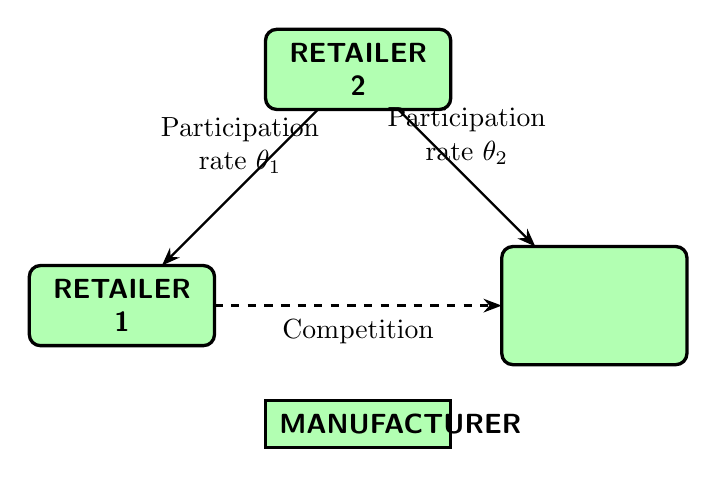
\begin{tikzpicture}[
    node distance=2cm and 3cm,
    every node/.style={inner sep=5pt, outer sep=0pt},
    retailer/.style={rectangle, rounded corners, draw=black, very thick, fill=green!30, text width=2cm, align=center, font=\sffamily\bfseries},
    manufacturer/.style={rectangle, draw=black, very thick, fill=green!30, text width=2cm, align=center, font=\sffamily\bfseries},
    participation/.style={->, >=Stealth, thick},
    competition/.style={->, >=Stealth, dashed, thick}
]

% Place nodes
\node (retailer2) [retailer] at (0, 0) {RETAILER 2};
\node (retailer1) [retailer] at (-3, -3) {RETAILER 1};
\node (retailer3) [retailer, draw=black, fill=green!30, minimum width=1.5cm, minimum height=1.5cm] at (3, -3) {};
\node (manufacturer) [manufacturer] at (0, -4.5) {MANUFACTURER};

% Draw participation arrows
\draw [participation] (retailer2) -- node[above, align=center] {Participation\\rate $\theta_1$} (retailer1);
\draw [participation] (retailer2) -- node[above, align=center] {Participation\\rate $\theta_2$} (retailer3);

% Draw competition arrow
\draw [competition] (retailer1) to[out=0, in=180, looseness=1.5] node[below, align=center] {Competition} (retailer3);

\end{tikzpicture}
\end{document}